% questions.tex —— 2004 年·天津卷·文科 · 题目内容片段（无答案）
% 由 tools/generate_projects.py 依来源总账自 2004/2004_数学真题_天津文_试题.md 生成，勿手改（改源 MD 后重跑）


\begin{gktip}
\textbf{来源说明}：本题面依据固定源 PDF 两页 A3 题面逐题转录，原卷印刷页码 204–205。固定源不附答案，答案和解析均由本库独立复算。

\textbf{图形说明}：第 8、11、19 题的原卷图形重绘为 TikZ 矢量图。
\end{gktip}

\gkpart{一、选择题（本大题共 12 小题，每小题 5 分，共 60 分．在每小题给出的四个选项中，只有一项是符合题目要求的）}

\begin{question}
\gkti{1}设集合 $P = \{1, 2, 3, 4, 5, 6\}$，$Q = \{x \in \mathbf{R} \mid 2 \le x \le 6\}$，那么下列结论正确的是\mbox{（　　）}

\begin{gkopts}(2)
\task A．$P \cap Q = P$
\task B．$P \cap Q \supseteq Q$
\task C．$P \cup Q = Q$
\task D．$P \cap Q \subsetneq P$
\end{gkopts}

\end{question}
\begin{question}
\gkti{2}不等式 $\dfrac{x-1}{x} \ge 2$ 的解集为\mbox{（　　）}

\begin{gkopts}(2)
\task A．$[-1, 0)$
\task B．$[-1, +\infty)$
\task C．$(-\infty, -1]$
\task D．$(-\infty, -1] \cup (0, +\infty)$
\end{gkopts}

\end{question}
\begin{question}
\gkti{3}对任意实数 $a, b, c$，在下列命题中，真命题是\mbox{（　　）}

\begin{gkopts}(2)
\task A．“$ac > bc$”是“$a > b$”的必要条件
\task B．“$ac = bc$”是“$a = b$”的必要条件
\task C．“$ac > bc$”是“$a > b$”的充分条件
\task D．“$ac = bc$”是“$a = b$”的充分条件
\end{gkopts}

\end{question}
\begin{question}
\gkti{4}若平面向量 $\vec{b}$ 与向量 $\vec{a} = (1, -2)$ 的夹角是 $180^\circ$，且 $|\vec{b}| = 3\sqrt{5}$，则 $\vec{b} =$\mbox{（　　）}

\begin{gkopts}(4)
\task A．$(-3, 6)$
\task B．$(3, -6)$
\task C．$(6, -3)$
\task D．$(-6, 3)$
\end{gkopts}

\end{question}
\begin{question}
\gkti{5}设 $P$ 是双曲线 $\dfrac{x^2}{a^2} - \dfrac{y^2}{9} = 1$ 上一点，双曲线的一条渐近线方程为 $3x - 2y = 0$，$F_1$、$F_2$ 分别是双曲线的左、右焦点，若 $|PF_1| = 3$，则 $|PF_2| =$\mbox{（　　）}

\begin{gkopts}(2)
\task A．$1$ 或 $5$
\task B．$6$
\task C．$7$
\task D．$9$
\end{gkopts}

\end{question}
\begin{question}
\gkti{6}若函数 $f(x) = \log_a x$ ($0 < a < 1$) 在区间 $[a, 2a]$ 上的最大值是最小值的 3 倍，则 $a =$\mbox{（　　）}

\begin{gkopts}(2)
\task A．$\dfrac{\sqrt{2}}{4}$
\task B．$\dfrac{\sqrt{2}}{2}$
\task C．$\dfrac{1}{4}$
\task D．$\dfrac{1}{2}$
\end{gkopts}

\end{question}
\begin{question}
\gkti{7}若过定点 $M(-1, 0)$ 且斜率为 $k$ 的直线与圆 $x^2 + 4x + y^2 - 5 = 0$ 在第一象限内的部分有交点，则 $k$ 的取值范围是\mbox{（　　）}

\begin{gkopts}(2)
\task A．$0 < k < \sqrt{5}$
\task B．$-\sqrt{5} < k < 0$
\task C．$0 < k < \sqrt{13}$
\task D．$0 < k < 5$
\end{gkopts}

\Needspace{0.4\textheight}
\end{question}
\begin{question}
\gkti{8}如图，定点 $A$ 和 $B$ 都在平面 $\alpha$ 内，定点 $P \notin \alpha$，$PB \perp \alpha$，$C$ 是 $\alpha$ 内异于 $A$ 和 $B$ 的动点，且 $PC \perp AC$．那么，动点 $C$ 在平面 $\alpha$ 内的轨迹是\mbox{（　　）}
\nopagebreak[4]
\begin{center}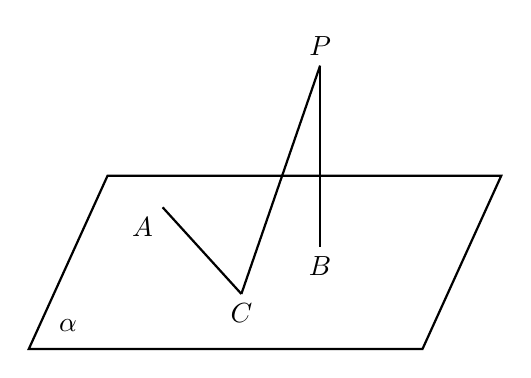
\begin{tikzpicture}[>=stealth, scale=1.0]
  % 平面 alpha
  \coordinate (M1) at (-0.5, -0.4);
  \coordinate (M2) at (4.5, -0.4);
  \coordinate (M3) at (5.5, 1.8);
  \coordinate (M4) at (0.5, 1.8);
  \draw[thick] (M1) -- (M2) -- (M3) -- (M4) -- cycle;
  \node at (0.0, -0.1) {$\alpha$};

  % 点坐标
  \coordinate (A) at (1.2, 1.4);
  \coordinate (B) at (3.2, 0.9);
  \coordinate (P) at (3.2, 3.2);
  \coordinate (C) at (2.2, 0.3);

  % 线段
  \draw[thick] (P) -- (B);
  \draw[thick] (P) -- (C);
  \draw[thick] (A) -- (C);

  % 节点标注
  \node[above] at (P) {$P$};
  \node[below] at (B) {$B$};
  \node[below left] at (A) {$A$};
  \node[below] at (C) {$C$};
\end{tikzpicture}
\end{center}
\nopagebreak[4]
\begin{gkopts}(2)
\task A．一条线段，但要去掉两个点
\task B．一个圆，但要去掉两个点
\task C．一个椭圆，但要去掉两个点
\task D．半圆，但要去掉两个点
\end{gkopts}

\end{question}
\begin{question}
\gkti{9}函数 $y = 3^{x^2 - 1}$ ($-1 \le x < 0$) 的反函数是\mbox{（　　）}

\begin{gkopts}(1)
\task A．$y = \sqrt{1 + \log_3 x}$ ($x \ge \dfrac{1}{3}$)
\task B．$y = -\sqrt{1 + \log_3 x}$ ($x \ge \dfrac{1}{3}$)
\task C．$y = \sqrt{1 + \log_3 x}$ ($\dfrac{1}{3} < x \le 1$)
\task D．$y = -\sqrt{1 + \log_3 x}$ ($\dfrac{1}{3} < x \le 1$)
\end{gkopts}

\end{question}
\begin{question}
\gkti{10}函数 $y = 2\sin\left(\dfrac{\pi}{6} - 2x\right)$ ($x \in [0, \pi]$) 为增函数的区间是\mbox{（　　）}

\begin{gkopts}(1)
\task A．$\left[0, \dfrac{\pi}{3}\right]$
\task B．$\left[\dfrac{\pi}{12}, \dfrac{7\pi}{12}\right]$
\task C．$\left[\dfrac{\pi}{3}, \dfrac{5\pi}{6}\right]$
\task D．$\left[\dfrac{5\pi}{6}, \pi\right]$
\end{gkopts}

\Needspace{0.4\textheight}
\end{question}
\begin{question}
\gkti{11}如图，在长方体 $ABCD - A_1B_1C_1D_1$ 中，$AB = 6, AD = 4, AA_1 = 3$．分别过 $BC$、$A_1D_1$ 的两个平行截面将长方体分成三部分，其体积分别记为 $V_1 = V_{AEA_1-DFD_1}$，$V_2 = V_{EBE_1A_1-FCF_1D_1}$，$V_3 = V_{B_1E_1B-C_1F_1C}$．若 $V_1 : V_2 : V_3 = 1 : 4 : 1$，则截面 $A_1EFD_1$ 的面积为\mbox{（　　）}
\nopagebreak[4]
\begin{center}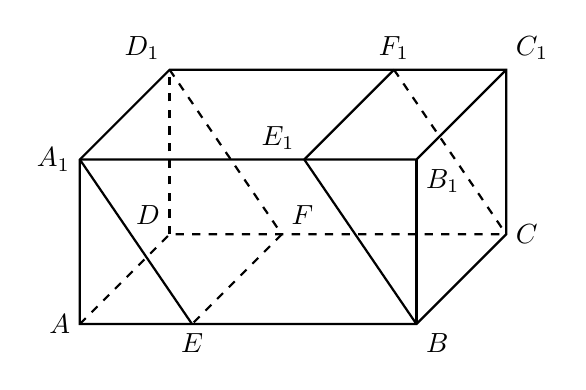
\begin{tikzpicture}[>=stealth, scale=0.95]
  % 顶点坐标
  \coordinate (A) at (0, 0);
  \coordinate (B) at (4.5, 0);
  \coordinate (C) at (5.7, 1.2);
  \coordinate (D) at (1.2, 1.2);

  \coordinate (A1) at (0, 2.2);
  \coordinate (B1) at (4.5, 2.2);
  \coordinate (C1) at (5.7, 3.4);
  \coordinate (D1) at (1.2, 3.4);

  % 截面分点 E, F, E1, F1 (比例 1:4:1, 即 1/6 与 5/6 处)
  % AB 长 4.5, E 在 1/3 (1.5) 处
  \coordinate (E) at (1.5, 0);
  \coordinate (F) at (2.7, 1.2);
  \coordinate (E1) at (3.0, 2.2);
  \coordinate (F1) at (4.2, 3.4);

  % 可见外框与实线
  \draw[thick] (A) -- (B) -- (C) -- (C1) -- (D1) -- (A1) -- cycle;
  \draw[thick] (A1) -- (B1) -- (C1);
  \draw[thick] (B) -- (B1);

  % 截面可见线
  \draw[thick] (A1) -- (E);
  \draw[thick] (E1) -- (B);
  \draw[thick] (E1) -- (F1);

  % 虚线（内部与被遮挡线）
  \draw[dashed, thick] (A) -- (D) -- (C);
  \draw[dashed, thick] (D) -- (D1);
  \draw[dashed, thick] (D1) -- (F) -- (E);
  \draw[dashed, thick] (F1) -- (C);

  % 节点标注
  \node[left] at (A) {$A$};
  \node[below right] at (B) {$B$};
  \node[right] at (C) {$C$};
  \node[above left] at (D) {$D$};

  \node[left] at (A1) {$A_1$};
  \node[below right] at (B1) {$B_1$};
  \node[above right] at (C1) {$C_1$};
  \node[above left] at (D1) {$D_1$};

  \node[below] at (E) {$E$};
  \node[above right] at (F) {$F$};
  \node[above left] at (E1) {$E_1$};
  \node[above] at (F1) {$F_1$};
\end{tikzpicture}
\end{center}
\nopagebreak[4]
\begin{gkopts}(4)
\task A．$4\sqrt{10}$
\task B．$8\sqrt{3}$
\task C．$4\sqrt{13}$
\task D．$16$
\end{gkopts}

\end{question}
\begin{question}
\gkti{12}定义在 $\mathbf{R}$ 上的函数 $f(x)$ 既是偶函数又是周期函数，若 $f(x)$ 的最小正周期是 $\pi$，且当 $x \in \left[0, \dfrac{\pi}{2}\right]$ 时，$f(x) = \sin x$，则 $f\left(\dfrac{5\pi}{3}\right)$ 的值为\mbox{（　　）}

\begin{gkopts}(2)
\task A．$-\dfrac{1}{2}$
\task B．$\dfrac{1}{2}$
\task C．$-\dfrac{\sqrt{3}}{2}$
\task D．$\dfrac{\sqrt{3}}{2}$
\end{gkopts}

\end{question}
\gkpart{二、填空题（本大题共 4 小题，每小题 4 分，共 16 分．把答案填在题中横线上）}

\begin{question}
\gkti{13}某工厂生产 A、B、C 三种不同型号的产品，产品数量之比依次为 $2 : 3 : 5$，现用分层抽样方法抽出一个容量为 $n$ 的样本，样本中 A 种型号产品有 16 件．那么此样本的容量 $n = \underline{\hspace{3em}}$．

\end{question}
\begin{question}
\gkti{14}已知向量 $\vec{a} = (1, 1), \vec{b} = (2, -3)$，若 $k\vec{a} - 2\vec{b}$ 与 $\vec{a}$ 垂直，则实数 $k$ 等于 $\underline{\hspace{3em}}$．

\end{question}
\begin{question}
\gkti{15}如果过两点 $A(a, 0)$ 和 $B(0, a)$ 的直线与抛物线 $y = x^2 - 2x - 3$ 没有交点，那么实数 $a$ 的取值范围是 $\underline{\hspace{3em}}$．

\end{question}
\begin{question}
\gkti{16}从 0, 1, 2, 3, 4, 5 中任取 3 个数字，组成没有重复数字的三位数，其中能被 5 整除的三位数共有 $\underline{\hspace{3em}}$ 个．（用数字作答）

\end{question}
\gkpart{三、解答题（本大题共 6 小题，共 74 分．解答应写出文字说明、证明过程或演算步骤）}

\begin{question}
\gkti{17}\textbf{（本小题满分 12 分）} 
已知 $\tan\left(\dfrac{\pi}{4} + \alpha\right) = \dfrac{1}{2}$．
（1）求 $\tan\alpha$ 的值；
（2）求 $\dfrac{\sin 2\alpha - \cos^2\alpha}{1 + \cos 2\alpha}$ 的值．

\end{question}
\begin{question}
\gkti{18}\textbf{（本小题满分 12 分）} 
从 4 名男生和 2 名女生中任选 3 人参加演讲比赛．
（1）求所选 3 人都是男生的概率；
（2）求所选 3 人中恰有 1 名女生的概率；
（3）求所选 3 人中至少有 1 名女生的概率．

\Needspace{0.4\textheight}
\end{question}
\begin{question}
\gkti{19}\textbf{（本小题满分 12 分）} 
如图，在四棱锥 $P - ABCD$ 中，底面 $ABCD$ 是正方形，侧棱 $PD \perp \text{\text{底面} } ABCD$，$PD = DC$，$E$ 是 $PC$ 的中点．
（1）证明：$PA \parallel \text{\text{平面} } EDB$；
（2）求 $EB$ 与底面 $ABCD$ 所成角的正切值．
\nopagebreak[4]
\begin{center}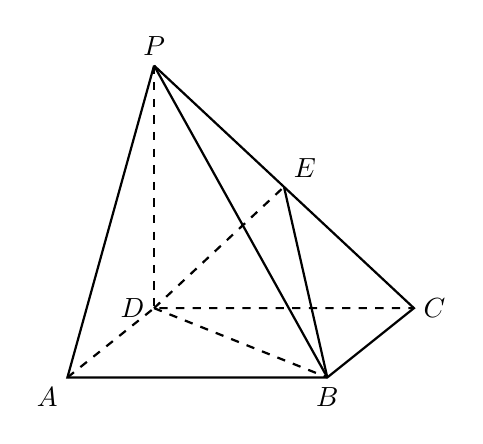
\begin{tikzpicture}[>=stealth, scale=1.1]
  % 顶点坐标
  \coordinate (D) at (1.0, 0.8);
  \coordinate (A) at (0, 0);
  \coordinate (B) at (3.0, 0);
  \coordinate (C) at (4.0, 0.8);
  \coordinate (P) at (1.0, 3.6);

  % 中点 E (PC 中点): P(1.0, 3.6), C(4.0, 0.8) -> E(2.5, 2.2)
  \coordinate (E) at (2.5, 2.2);

  % 实线棱
  \draw[thick] (P) -- (A) -- (B) -- (C) -- (P);
  \draw[thick] (P) -- (B);
  \draw[thick] (E) -- (B);

  % 虚线棱与辅助线
  \draw[dashed, thick] (P) -- (D);
  \draw[dashed, thick] (A) -- (D) -- (C);
  \draw[dashed, thick] (D) -- (B);
  \draw[dashed, thick] (D) -- (E);

  % 节点标注
  \node[above] at (P) {$P$};
  \node[below left] at (A) {$A$};
  \node[below] at (B) {$B$};
  \node[right] at (C) {$C$};
  \node[left] at (D) {$D$};
  \node[above right] at (E) {$E$};
\end{tikzpicture}
\end{center}
\nopagebreak[4]
\end{question}
\begin{question}
\gkti{20}\textbf{（本小题满分 12 分）} 
设 $\{a_n\}$ 是一个公差为 $d$ ($d \ne 0$) 的等差数列，它的前 10 项和 $S_{10} = 110$，且 $a_1, a_2, a_4$ 成等比数列．
（1）证明：$a_1 = d$；
（2）求公差 $d$ 的值和数列 $\{a_n\}$ 的通项公式．

\end{question}
\begin{question}
\gkti{21}\textbf{（本小题满分 12 分）} 
已知函数 $f(x) = ax^3 + cx + d$ ($a \ne 0$) 是 $\mathbf{R}$ 上的奇函数，当 $x = 1$ 时 $f(x)$ 取得极值 $-2$．
（1）求 $f(x)$ 的单调区间和极大值；
（2）证明：对任意 $x_1, x_2 \in (-1, 1)$，不等式 $|f(x_1) - f(x_2)| < 4$ 恒成立．

\end{question}
\begin{question}
\gkti{22}\textbf{（本小题满分 14 分）} 
椭圆的中心是原点 $O$，它的短轴长为 $2\sqrt{2}$，相应于焦点 $F(c, 0)$ ($c > 0$) 的准线 $l$ 与 $x$ 轴相交于点 $A$，$|OF| = 2|FA|$，过点 $A$ 的直线与椭圆相交于 $P$、$Q$ 两点．
（1）求椭圆的方程及离心率；
（2）若 $\vec{OP} \cdot \vec{OQ} = 0$，求直线 $PQ$ 的方程．

\end{question}